\documentclass[10pt,c]{beamer}

\usepackage[english,french]{babel}
\usepackage[T1]{fontenc}
\usepackage[utf8]{inputenc}
\usepackage{graphicx}
\usepackage{multirow}


%%%%%%%%%%%%%%%%%%%%%%%%%%%%%%%%%%%%%%%%%%%%%%%%%%%%%%%%%%%%%%%%%%%%%%%%%%%%%%%%
%%%                               80 COLONNES                                %%%
%%%%%%%%%%%%%%%%%%%%%%%%%%%%%%%%%%%%%%%%%%%%%%%%%%%%%%%%%%%%%%%%%%%%%%%%%%%%%%%%

%%% THÈME DE LA PRÉSENTATION
\usetheme{Warsaw}

%%% ÉLÉMENTS DE TITRE
\title[Évaluation et amélioration des PF logicielles...]
      {Évaluation et amélioration des plates-formes logicielles
       pour réseaux de capteurs sans-fil, pour optimiser la
       qualité de service et l'énergie}
\author{Kévin Roussel}
\institute{INRIA Nancy Grand-Est~---
           LORIA UMR~7503~--- Université de Lorraine \\
           \vspace{0.25cm}
           \textit{Directeurs de thèse~: Ye-Qiong SONG et Olivier ZENDRA}}
\date{3~juin 2016}


%%%%%%%%%%%%%%%%%%%%%%%%%%%%%%%%%%%%%%%%%%%%%%%%%%%%%%%%%%%%%%%%%%%%%%%%%%%%%%%%
%%%                               80 COLONNES                                %%%
%%%%%%%%%%%%%%%%%%%%%%%%%%%%%%%%%%%%%%%%%%%%%%%%%%%%%%%%%%%%%%%%%%%%%%%%%%%%%%%%

%%% COMMANDES UTILES AU COURS DU CORPS DE TEXTE

\newcommand{\lang}[1]{\textit{#1}}
\newcommand{\nom}[1]{\textbf{#1}}
\renewcommand{\emph}[1]{\textbf{\textit{#1}}}
\newcommand{\flcaption}[1]{\caption{\textsl{#1}}}

\setbeamertemplate{itemize item}[triangle]
\setbeamertemplate{itemize subitem}[square]
\setbeamertemplate{itemize subsubitem}[circle]
\setbeamertemplate{bibliography item}{\insertbiblabel}
% Ajout des numéros de transparents à la barre de navigation en bas à droite
\setbeamercolor{footline}{fg=darkgray}
\setbeamerfont{footline}{series=\bfseries,size=\scriptsize}
\setbeamertemplate{navigation symbols}{%
    \usebeamerfont{footline}%
    \usebeamercolor[fg]{footline}%
    \hspace{1.5em}%
    \insertframenumber~/ \insertpresentationendpage
}
% Augmenter la taille des "balles" des sections dans les sommaires
\pgfdeclareradialshading{blueball}{\pgfpoint{0.5mm}{0.5mm}}{%
  rgb(0mm)=(0,0,0.9);
  rgb(0.7mm)=(0,0,0.7);
  rgb(1mm)=(0,0,0.5);
  rgb(1.05mm)=(1,1,1)
}
\defbeamertemplate{section in toc}{largeball}{%
  \begin{pgfpicture}{-1ex}{-0.65ex}{1.5ex}{1.5ex}%
  \usebeamercolor[fg]{item projected}%
  {\pgftransformscale{2.5}\pgftext{\normalsize\pgfuseshading{blueball}}}%
  {\pgftransformshift{\pgfpoint{0pt}{0.5pt}}%
  \pgftext{\usebeamerfont*{item projected}%
           \large\inserttocsectionnumber}}%
  \end{pgfpicture}%
  \hspace{1.5mm}\inserttocsection
}
\setbeamertemplate{section in toc}[largeball]
% Augmenter la taille des "balles" des listes énumérées
\defbeamertemplate{enumerate item}{largeball}{%
  \begin{pgfpicture}{-1ex}{-0.65ex}{1.5ex}{1.5ex}%
  \usebeamercolor[fg]{item projected}%
  {\pgftransformscale{1.75}\pgftext{\scriptsize\pgfuseshading{blueball}}}%
  {\pgftransformshift{\pgfpoint{0pt}{0.5pt}}%
  \pgftext{\usebeamerfont*{item projected}\normalsize\insertenumlabel}}%
  \end{pgfpicture}%
}
\setbeamertemplate{enumerate item}[largeball]
% Réutiliser les "balles de listes énumérées dans le texte
\newcommand{\circleddigit}[1]{%
  {\renewcommand{\insertenumlabel}{#1}\usebeamertemplate{enumerate item}}%
}


%%%%%%%%%%%%%%%%%%%%%%%%%%%%%%%%%%%%%%%%%%%%%%%%%%%%%%%%%%%%%%%%%%%%%%%%%%%%%%%%
%%%                               80 COLONNES                                %%%
%%%%%%%%%%%%%%%%%%%%%%%%%%%%%%%%%%%%%%%%%%%%%%%%%%%%%%%%%%%%%%%%%%%%%%%%%%%%%%%%

%%% DÉBUT DE LA PRÉSENTATION
\begin{document}

%%% TITRE
\begin{frame}
\titlepage
\end{frame}

%%% MACRO : SOUS-SOMMAIRE POUR CHAQUE SECTION
\AtBeginSection[]
{
  \begin{frame}
  \frametitle{\secname~--- sommaire}
  \tableofcontents[currentsection, hideothersubsections,
                   sectionstyle=show/hide]
  \end{frame}
}

\part{debut}

%%%%%%%%%%%%%%%%%%%%%%%%%%%%%%%%%%%%%%%%%%%%%%%%%%%%%%%%%%%%%%%%%%%%%%%%%%%%%

%%% SECTION 1 : INTRODUCTION
\section{Introduction}

\begin{frame}[label=intro1]
\frametitle{Introduction I}

\begin{block}{Réseaux de capteurs sans-fil (WSN)}
\begin{itemize}
\item Constitués de n{\oe}uds nommés \nom{capteurs sans-fil}
      ou \lang{``motes''}
\item Interconnexion entre eux $\rightarrow$ \emph{Internet of Things (IoT)}
\end{itemize}
\end{block}

\begin{block}{Plates-formes logicielles (OS) spécialisées dans les WSN}
\begin{itemize}
\item ... avec \nom{piles protocolaires réseau} spécialisées
\item \emph{Maillon faible = couches basses de ces piles réseau} \\
      {\small (comme nous allons le démontrer)}
\end{itemize}
\end{block}

\end{frame}

\begin{frame}[label=intro2]
\frametitle{Introduction II}

\begin{columns}[c]
\begin{column}{8.5cm}

\begin{alertblock}{\large\textbf{But de la thèse~:}}
\large\emph{Développer des méthodes pour améliorer ces couches basses,
en exploitant toutes les fonctionnalités offertes par ces OS dédiés}
\end{alertblock}

\end{column}
\end{columns}

\end{frame}

%%%%%%%%%%%%%%%%%%%%%%%%%%%%%%%%%%%%%%%%%%%%%%%%%%%%%%%%%%%%%%%%%%%%%%%%%%%%%

%%% SECTION 2 : CONTEXTE ET PROBLÉMATIQUE
\section{Contexte et problématique}


%% 2.1 : CONTEXTE
\subsection{Contexte}

\begin{frame}[label=contexte1]
\frametitle{Contexte~: applications d'e-santé des WSN}
\framesubtitle{Un domaine déjà bien établi et très actif}

\vspace{-0.5cm}

\begin{columns}[c]

\begin{column}{7cm}

\center{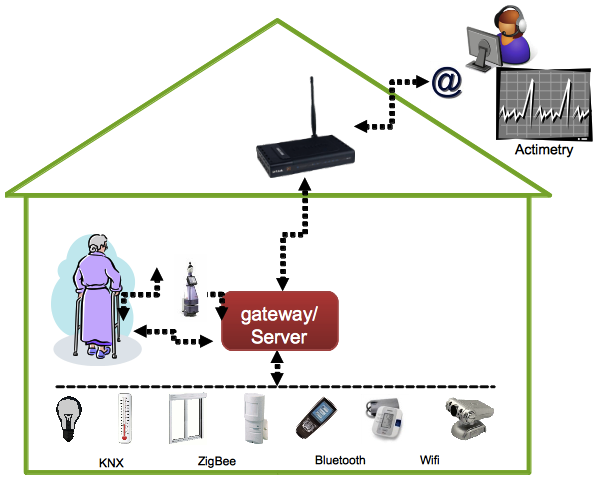
\includegraphics[width=7cm]{images/projet-lar-resume.png}}

\end{column}

\begin{column}{4cm}

\begin{alertblock}{Le projet \nom{LAR}~: \lang{``Living Assistant Robot''}}

But~: aider au maintien à domicile des personnes âgées~/ dépendantes,
en retardant au maximum leur placement en institutions spécialisées. \\

$\rightarrow$ Financement de la présente thèse.
\end{alertblock}

\end{column}

\end{columns}

\end{frame}


%% 2.2 : PROBLÉMATIQUE
\subsection{Problématique}

\begin{frame}[label=problematique1]
\frametitle{Problématique de la thèse}
\framesubtitle{Couches des piles protocolaires réseau dédiées aux WSN}

\vspace{-0.25cm}

\begin{block}{Deux extrêmités dans les piles réseau pour WSN~/ IoT~:}
\begin{itemize}
\item Les couches hautes (routage, applications, Web des objets, etc.) \\ 
      $\rightarrow$ nombreux travaux réalisés et publiés
\item Les couches basses (physique~/ pilotes radio, MAC~/
       RDC\footnotemark[1]) \\ 
      $\rightarrow$ pas d'implémentations \emph{à la fois} efficaces,
       portables et standardisées
\end{itemize}
\end{block}

\begin{block}{Faiblesses des couches basses~:}
\begin{itemize}
\item Sapent les fondations des travaux sur couches hautes
\item \emph{<<~Château bâti sur du sable~>>}
\end{itemize}
\end{block}

\footnotetext[1]{\scriptsize \nom{RDC~:} \lang{Radio Duty Cycle} (Cycle de
fonctionnement~--- activation et désactivation~--- \\ de l'émetteur~/
récepteur radio)}

\end{frame}


%% 2.3 : POSTULATS DE THÈSE
\subsection{Postulats}

\begin{frame}[label=postulats1]
\frametitle{Postulats de notre thèse}

\begin{alertblock}{\textbf{Notre Thèse}}
\emph{Une fondation solide pour l'IoT passe par le développement de~:}
\begin{itemize}
\item \emph{des protocoles MAC~/ RDC avancés à haute QdS\footnotemark[1],}
\item \emph{sur un OS dédié WSN~:}
  \begin{itemize}
  \item \emph{\normalsize reconnu et répandu,}
  \item \emph{\normalsize offrant les fonctionnalités requises (temps-réel).}
  \end{itemize}
\end{itemize}
\end{alertblock}

\footnotetext[1]{\scriptsize \nom{QdS~:} qualité de service
 \lang{(QoS~:Quality of Service)}}

\end{frame}

%%%%%%%%%%%%%%%%%%%%%%%%%%%%%%%%%%%%%%%%%%%%%%%%%%%%%%%%%%%%%%%%%%%%%%%%%%%%%

\part{principal}

%%% SOMMAIRE GÉNÉRAL

\section*{}

\begin{frame}
\frametitle{Sommaire général}
\vspace{-0.375cm}
\tableofcontents[part=1,hideallsubsections,sectionstyle=shaded]
\vspace{-0.1cm}
\tableofcontents[hideallsubsections]
\end{frame}

%%%%%%%%%%%%%%%%%%%%%%%%%%%%%%%%%%%%%%%%%%%%%%%%%%%%%%%%%%%%%%%%%%%%%%%%%%%%%

%%% SECTION 3 : ÉTAT DE L'ART
\section{Analyse critique de l'état de l'art}


%% 3.1 PROTOCOLE IEEE 802.15.4
\subsection{Le protocole IEEE 802.15.4}

\begin{frame}[label=ieeephys1]
\frametitle{Le protocole IEEE 802.15.4}

\nom{Protocole 802.15.4}~: ne concerne que les deux couches les plus basses
(1~--- PHY \& 2~--- MAC)

\vspace{-0.25cm}
\center{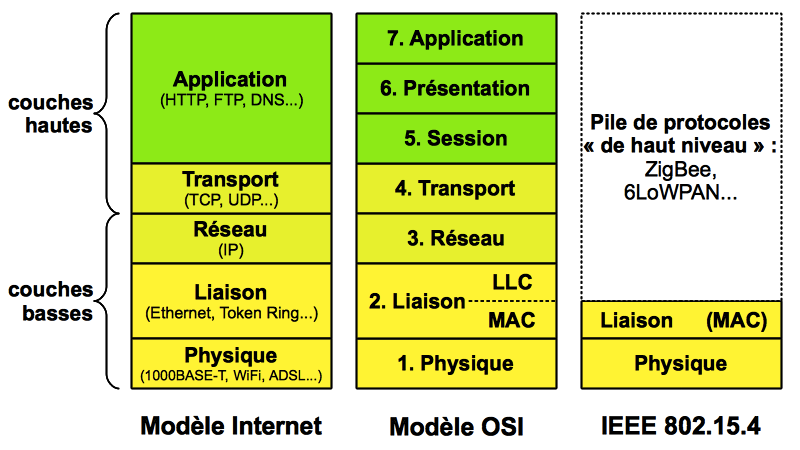
\includegraphics[height=5.25cm]{images/ip-vs-osi-vs-802154.png}}

\end{frame}


%% 3.2 PROTOCOLES MAC / RDC
\subsection{Protocoles MAC~/ RDC}

\begin{frame}[label=protoMACRDC1]
\frametitle{Protocoles MAC I}
\framesubtitle{Difficulté~: synchronisation (points de rendez-vous)
entre n{\oe}uds avec des \lang{duty cycles} différents}

\vspace{-0.25cm}
\begin{block}{Nombreux protocoles MAC alternatifs}
Basés sur différentes approches~:
\begin{itemize}
\item Contention (CSMA/CA)\footnotemark[1]~:
  \begin{itemize}
  \item Synchrones
  \item Asynchrones~:
    \begin{itemize}
    \item \'Ecoute à basse énergie
           (LPL~: \lang{Low-Power Listening}) \\
           $\rightarrow$ SI~: \lang{Sender-Initiated}
    \item \'Emission à basse énergie
           (LPP~: \lang{Low-Power Probing}) \\
           $\rightarrow$ RI~: \lang{Receiver-Initiated}
    \end{itemize}
  \end{itemize}
\item Multiplexage~:
  \begin{itemize}
  \item Temporel
         {\footnotesize(TDMA~: \lang{Time Division Multiple Access})}
  \item Fréquentiel
         {\footnotesize(FDMA~: \lang{Frequency Division Multiple Access})}
  \end{itemize}
\item Hybrides
\end{itemize}
\end{block}

\footnotetext[1]{\scriptsize \nom{CSMA/CA~:} \lang{Carrier Sense Multiple
Access with Collision Avoidance} (\'Ecoute d'un Support à Accès Multiple,
avec \'Evitement des Collisions)}

\end{frame}

\begin{frame}[label=protoMACRDC2]
\frametitle{Protocoles MAC II}

Exemple de protocole MAC~/ RDC classique et très utilisé~: \nom{ContikiMAC}

\center{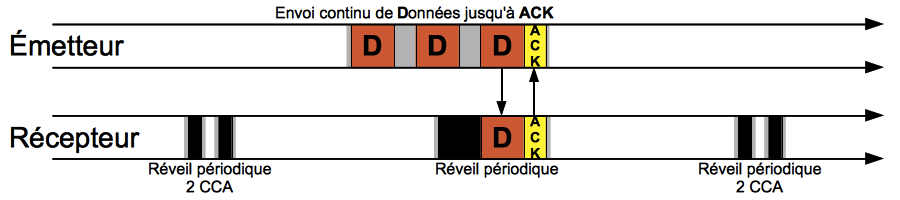
\includegraphics[width=10.75cm]{images/contikimac.png}}

\begin{itemize}
\item Basé sur la contention (CSMA~/ CA, paradigme LPL)
\item Cycle de fonctionnement fixe (défini à la compilation),
correspondant au délai entre deux écoutes successives du médium radio \\ 
$\rightarrow$ Adaptation <<~réactive~>> au trafic {\small(écoute tant que
médium occupé)} \\
+ optimisation récente~: \lang{``phase lock''}
\end{itemize}

\end{frame}

\begin{frame}[label=protoMACRDC3]
\frametitle{Protocoles MAC III}

\vspace{-0.25cm}

Exemple de protocole MAC~/ RDC avancé~: \nom{S-CoSenS}

\begin{itemize}
\item Adaptation \emph{calculée} au trafic radio~:
\end{itemize}

\centering{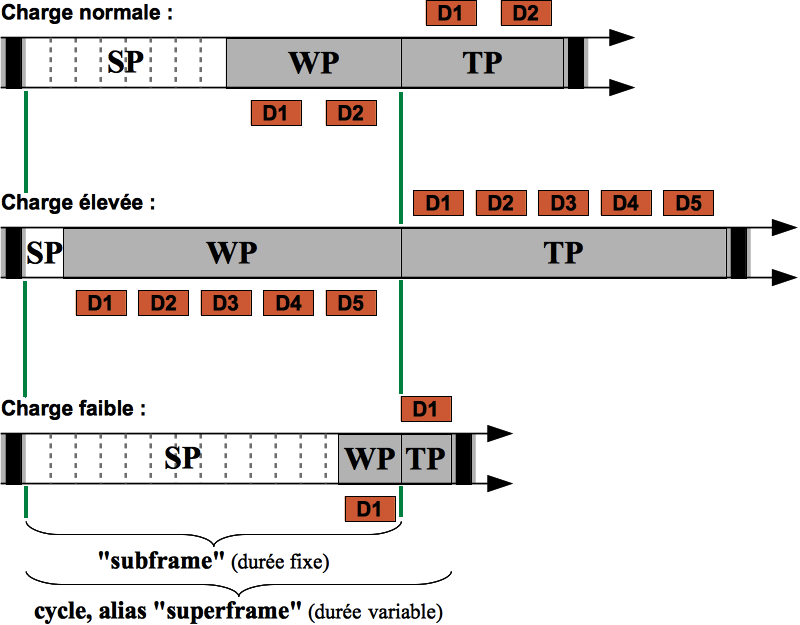
\includegraphics[width=6.5cm]{images/s-cosens-cycle.png}}

\end{frame}

\begin{frame}[label=protoMACRDC4]
\frametitle{Protocoles MAC IV}

\vspace{-0.25cm}

Exemple de protocole MAC~/ RDC avancé~: \nom{S-CoSenS} (suite et fin)

\begin{itemize}
\item Contention, hybride LPP~/ LPL~:
  \begin{itemize}
  \item LPP (RI) $\rightarrow$ communication intra-PAN\footnotemark[1]
  \item LPL $\rightarrow$ communication entre routeurs (inter-PAN)
  \end{itemize}
\item Transmission d'un paquet~:
\end{itemize}

\centering{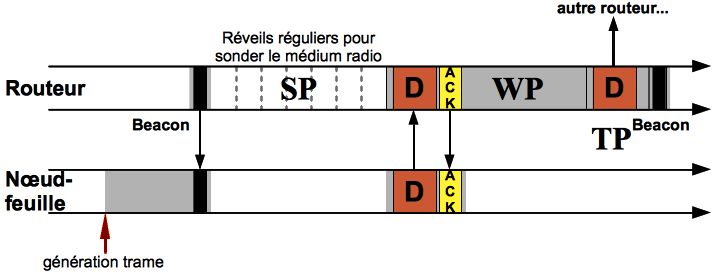
\includegraphics[width=8cm]{images/s-cosens-transmission.png}}

\footnotetext[1]{\scriptsize \nom{PAN~:} \lang{Personal Area Network}
(Réseau d'\'Etendue Personnelle~; réseau élémentaire dans \\
le domaine des WSN)}

\end{frame}

\begin{frame}[label=protoMACRDC5]
\frametitle{Protocoles MAC V}
\framesubtitle{Synthèse sur les protocoles MAC~/ RDC}

\vspace{-0.25cm}
\begin{block}{Différence fondamentale entre protocoles <<~classiques~>>
              et <<~avancés~>>}
Adaptation au trafic réseau~:
\begin{itemize}
\item protocoles <<~classiques~>> (802.15.4[e], ContikiMAC...)~:
 \emph{configuration statique ou adaptation réactive par essai~/ erreur} \\
{\footnotesize (allongement de la période active en cas de trafic
  pour ContikiMAC)}
\item protocoles <<~avancés~>> (S-CoSenS, iQueueMAC...)~: \\
 \emph{adaptation proactive par calcul des besoins} au trafic réseau \\
{\footnotesize (par mesure ou estimation de l'intensité de ce trafic)}
\end{itemize}
\end{block}

\vspace{-0.25cm}
\begin{alertblock}{En résumé~:}
\begin{center}
\begin{tabular}{ccc}
\textbf{<<~classique~>>~= réactif} & \textbf{/} &
  \textbf{<<~avancé~>>~= proactif}
\end{tabular}
\end{center}
\end{alertblock}

\end{frame}


%% 3.3 OS DÉDIÉS
\subsection{Systèmes d'exploitation dédiés}

\begin{frame}[label=osDedies1]
\frametitle{Systèmes d'exploitation spécialisés I}

\begin{block}{Multiples OS développés pour les WSN}
Différences~:
\begin{itemize}
\item fonctionnalités offertes
\item exigences matérielles
\item diffusion~/ adoption
\end{itemize}
\end{block}

\end{frame}

\begin{frame}[label=osDedies2]
\frametitle{Systèmes d'exploitation spécialisés II}

Rappel sur les notions de multitâche et de temps-réel~:

\begin{columns}[b]

\begin{column}{6cm}

\center{
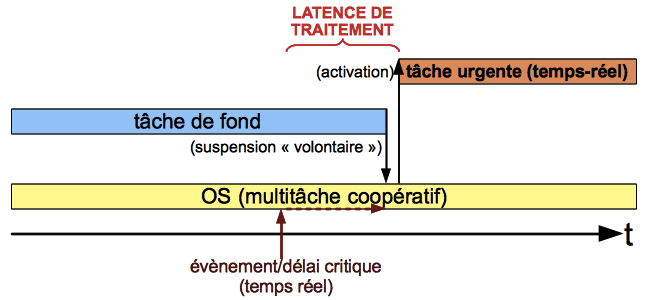
\includegraphics[width=6cm]{images/multitache-cooperatif.png}

\scriptsize Modèle multitâche \textbf{coopératif} et temps-réel
}

\end{column}

\begin{column}{6cm}

\center{
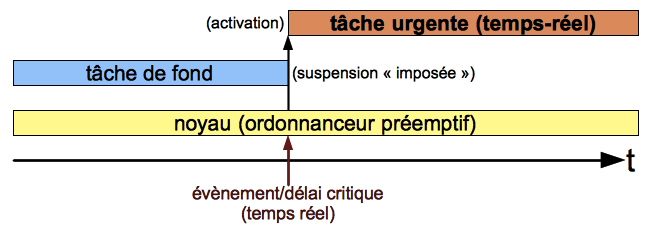
\includegraphics[width=6cm]{images/multitache-preemptif.png}

\scriptsize Modèle multitâche \textbf{préemptif} et temps-réel
}

\end{column}

\end{columns}

\end{frame}

\begin{frame}[label=osDedies3]
\frametitle{Systèmes d'exploitation spécialisés III}

\begin{tabular}{|c|c|c|}
\hline
\textbf{OS} & \textbf{Capacités}         & \textbf{Nous recommandons pour} \\
            &                            & \textbf{les protocoles...} \\
\hline
   TinyOS   & MT coopératif              & asynchrones \\
\hline
   Contiki  & MT coopératif,             & basés sur la contention \\
            &  temps-réel <<~basique~>>  & \\
\hline
   LiteOS   & MT préemptif               & basés sur la  contention \\
            &                            & \\
\hline
   NanoRK   & MT préemptif,              & tous~: contention, \\
            &  temps-réel                &  multiplexage, avancés \\
\hline
  RIOT OS   & MT préemptif,              & tous~: contention, \\
            &  temps-réel                &  multiplexage, avancés \\
\hline
  FreeRTOS  & \textit{Noyau} MT préemptif, & tous~: contention, \\
            &  temps-réel                  &  multiplexage, avancés \\
            &                              &  (OpenWSN) \\
\hline
\end{tabular}

\end{frame}

\begin{frame}[label=osDedies4]
\frametitle{Systèmes d'exploitation spécialisés IV}
\framesubtitle{Synthèse sur les OS pour WSN~: choix de PF logicielles}

\begin{block}{Plates-formes logicielles choisies~:}

\begin{itemize}
\item \nom{Contiki OS}~: référence actuelle dans le domaine des WSN~---
           standard de fait, au moins dans la recherche académique
\item \nom{RIOT OS}~: plate-forme très récente, performante~--- notamment
           sur les fonctionnalités temps-réel~---, et au développement
           dynamique et ouvert (auquel nous avons participé)
\end{itemize}

\end{block}

\end{frame}

%%%%%%%%%%%%%%%%%%%%%%%%%%%%%%%%%%%%%%%%%%%%%%%%%%%%%%%%%%%%%%%%%%%%%%%%%%%%%

%%% SECTION 4 : PLATES-FORMES LOGICIELLES : ÉVALUATION ET AMÉLIORATIONS
\section[Plates-formes logicielles]
        {Plates-formes logicielles~: évaluation, problèmes et améliorations}


%% 4.1 CONTIKI
\subsection{Contiki~: développement et limitations}

\begin{frame}[label=contiki1]
\frametitle{Contiki OS I}

\begin{exampleblock}{Contiki OS~: avantages}
\begin{itemize}
\item Standard de fait actuel~: très répandu et utilisé
\item Très peu gourmand en ressources matérielles
\item Nombreuses fonctionnalités réseau~: ContikiMAC, uIPv6, Rime...
\item Nombreux portages (architectures MCU\footnotemark[1] et matériels)
\item Codé en C {\small(avec quelques limitations)}
\item Fonctionne de base avec \nom{Cooja}~: simulateur~/ émulateur de WSN
\end{itemize}
\end{exampleblock}

\footnotetext[1]{\scriptsize \nom{MCU~:} \lang{MicroController Unit}
(Microcontrôleur)}

\end{frame}

\begin{frame}[label=contiki2]
\frametitle{Contiki OS II}

\vspace{-0.25cm}
\begin{alertblock}{Contiki OS~: limites bloquantes}
\begin{itemize}
\item Multitâche coopératif~: \lang{``protothreads''}
\item Documentation minimaliste
\item Limites techniques~:
  \begin{itemize}
  \item pilotes radio incomplets durant nos travaux\footnotemark[1]
  \item pile réseau centrée sur un unique \textsl{``\texttt{packetbuf}''}
  \item complexité excessive de la pile réseau
  \end{itemize}
\item Fonctionnalités temps-réel insuffisantes (\texttt{rtimer})~:
  \begin{itemize}
  \item une seule instance de \texttt{rtimer}
  \item code du système non réentrant
  \item sans \texttt{rtimer}~: granularité très insuffisante (8~ms)
  \end{itemize}
\item Coopération avec l'équipe de développement quasi-impossible
\end{itemize}
\end{alertblock}

\footnotetext[1]{\scriptsize (corrigé dans la \lang{release}~3.0)}

\end{frame}


%% 4.2 RIOT OS : DÉCOUVERTE ET CONTRIBUTIONS
\subsection{RIOT OS~: découverte et contributions}

\begin{frame}[label=RIOT1]
\frametitle{RIOT OS I}

\begin{exampleblock}{RIOT OS~: avantages}
\begin{itemize}
\item Micro-noyau à multitâche préemptif
\item Gestion avancée du temps-réel (avec fine granularité
       $\leadsto$ 1 $\mu$s)
\item Soin apporté à la qualité du code
\item Codé en C standard (ISO C 99) sans limitations
\item Architecture modulaire~: tout est optionnel hors micro-noyau
\item \'Equipe de développement ouverte et réactive
\end{itemize}
\end{exampleblock}

\end{frame}

\begin{frame}[label=RIOT2]
\frametitle{RIOT OS II}

\begin{block}{RIOT OS~: inconvénients}
\begin{itemize}
\item Projet récent~: premières versions publiées en 2013
\item Porté sur moins d'architectures MCU que, par exemple, Contiki~:
  \begin{itemize}
  \item ARM (v7~puis Cortex-M)
  \item MSP430
  \item AVR
  \end{itemize}
\item Développement rapide, mais encore <<~jeune~>> sur certains points~:
  \begin{itemize}
  \item API des \lang{timers} refaite~: \texttt{xtimer}
  \item Nouvelle pile protocolaire réseau~: \texttt{gnrc}
  \end{itemize}
 $\rightarrow$ nécessité de recoder les applications
\end{itemize}
\end{block}

\end{frame}

\begin{frame}[label=RIOT3]
\frametitle{RIOT OS III}

\vspace{-0.25cm}

\begin{exampleblock}{Contributions techniques (\lang{Pull Requests}
                     sur GitHub)}
\begin{itemize}
\item Gestion des erreurs fatales (\texttt{core\_panic()} ajoutée
       au noyau)
\item Portage de RIOT sur plate-forme matérielle Zolertia Z1
\item Déboguage de RIOT OS sur architecture MCU MSP430
\item Autres contributions {\small (déboguage et améliorations
       $\rightarrow\ \ \approx$ une trentaine)}
\end{itemize}
\end{exampleblock}

\begin{block}{Autre contribution}
Analyse critique de la nouvelle pile réseau (\texttt{gnrc}) de RIOT OS
\end{block}

\end{frame}

%%%%%%%%%%%%%%%%%%%%%%%%%%%%%%%%%%%%%%%%%%%%%%%%%%%%%%%%%%%%%%%%%%%%%%%%%%%%%

%%% SECTION 5 : ÉVALUATION ET COMPARAISON DE PROTOCOLES MAC / RDC
\section[Protocoles MAC~/RDC]
        {\'Evaluation et comparaison de protocoles MAC~/ RDC}


%% 5.1 PREMIÈRES PLATES-FORMES MATÉRIELLES
\subsection{Premières plates-formes matérielles}

\begin{frame}[label=pfMSP1]
\frametitle{Premières plates-formes matérielles}
\framesubtitle{TelosB~/ SkyMote et Zolertia Z1}

\vspace{-0.25cm}
\begin{block}{Premières plates-formes matérielles (surtout émulées)}
\begin{itemize}
\item Basées sur l'architecture MSP430~:
  \begin{itemize}
  \item MCU MSP430F1611 pour la TelosB~/ SkyMote \\
         {\small (8~MHz, 48~Ko Flash, 10~Ko RAM)}
  \item MCU MSP430F2617 pour la Zolertia Z1 \\
         {\small (16~MHz, 92~Ko Flash, 8~Ko RAM)}
  \end{itemize}
\item Même émetteur~/récepteur radio~: TI ChipCon CC2420
\item Divers capteurs physiques {\small (plus bus d'extension pour capteurs
      supplémentaires~--- \lang{``Phidgets''}~--- sur Zolertia Z1)}
\item En commun~: antenne intégrée, port pour antenne externe, \\
       mémoire Flash hors MCU (stockage permanent de données)
\end{itemize}
\end{block}

\end{frame}


%% 5.2 IMPLANTATION DE S-COSENS SOUS RIOT OS
\subsection[Implantation de S-CoSenS sous RIOT OS]
           {Implantation de S-CoSenS sous RIOT OS~:
            précision de la synchronisation entre n{\oe}uds}

\begin{frame}[label=implSCoSenS1]
\frametitle{Implantation de S-CoSenS sous RIOT OS I}

PAN virtual de test (schéma structurel)~:
\vspace{-0.35cm}
\center{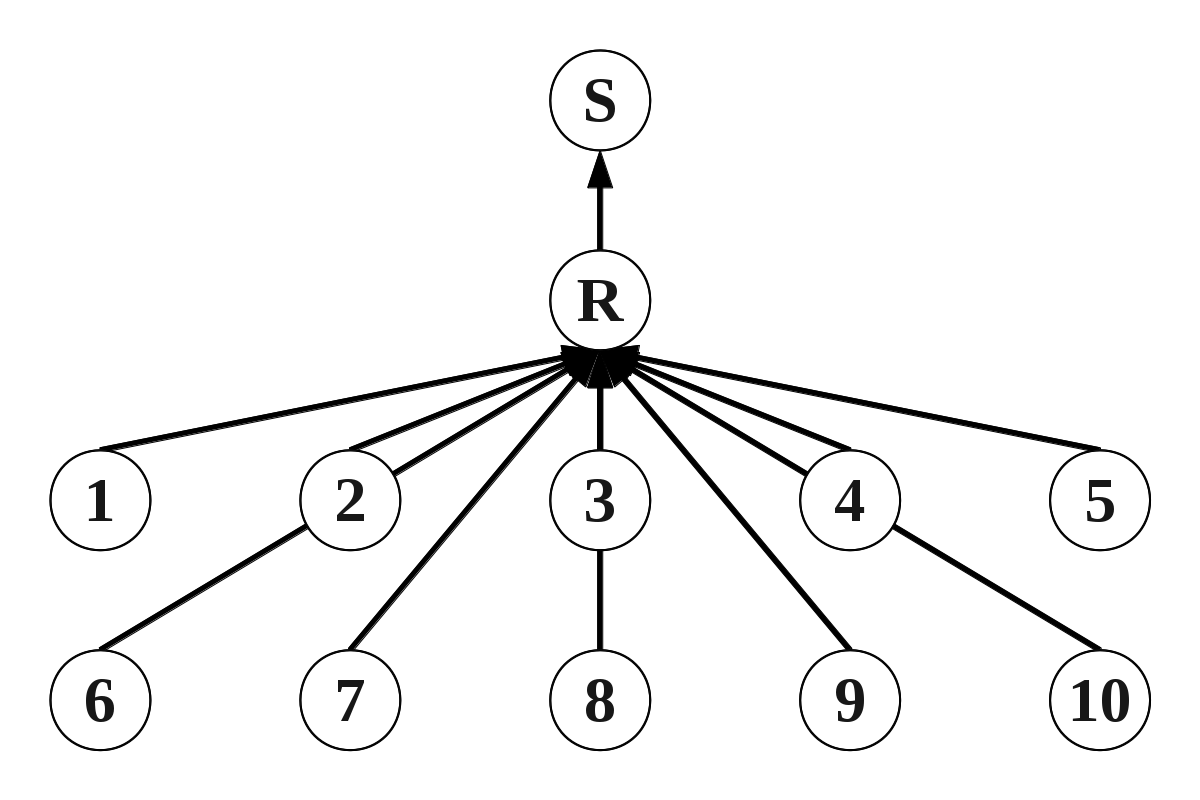
\includegraphics[width=8.5cm]{images/virtual-pan-test-1.png}}

\end{frame}

\begin{frame}[label=implSCoSenS2]
\frametitle{Implantation de S-CoSenS sous RIOT OS II}
\framesubtitle{Premier test sous Cooja}

Synchronisation précise et efficace entre n{\oe}uds, grâce aux
fonctionnalités temps-réel de RIOT OS~:
\center{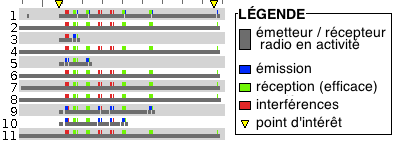
\includegraphics[width=10.5cm]{images/s-cosens-timeline-1.png}}

\end{frame}


%% 5.3 ÉVALUATION DES PERFORMANCES : COMPARAISON AVEC CONTIKIMAC
\subsection{\'Evaluation des performances~: comparaison avec ContikiMAC}

\begin{frame}[label=comparContikiMAC1]
\frametitle{Comparaison avec ContikiMAC I}
\framesubtitle{\'Evaluation: configuration des expériences}

Débit réseaux utiles programmés sur l'ensemble des dix n{\oe}uds-feuilles~:

\center{
\begin{tabular}{|l|r|r|r|}
\hline
\textbf{Configuration}
            & \textbf{PTI}\footnotemark[1] \textbf{moyen}
                      & \textbf{Fréquence TX}
                                         & \textbf{Débit total} \\
            & \textbf{(par n{\oe}ud)}
                      & \textbf{moyenne totale}
                                         & \textbf{attendu}\\
\hline
Modérée     & 1500 ms &   6,7 trames~/ s &  5867 bit~/ s \\
\'Elevée    & 1000 ms &    10 trames~/ s &  8800 bit~/ s \\
Très élevée &  500 ms &    20 trames~/ s & 17600 bit~/ s \\
Extrême     &  100 ms &   100 trames~/ s & 88000 bit~/ s \\
\hline
\end{tabular}
}

\raggedright\vspace{0.5cm}
File d'envoi d'une taille de 8 paquets pour tous les tests.

\footnotetext[1]{\vspace{0.25cm} \scriptsize \nom{PTI~:}
\lang{Packet Transmission Interval}, Intervalle d'\'Emission
des Paquets~/ trames}

\end{frame}

\begin{frame}[label=comparContikiMAC2]
\frametitle{Comparaison avec ContikiMAC II}
\framesubtitle{Qualité de service}

S-CoSenS~/ RIOT aussi bon ou meilleur que ContikiMAC~/ Contiki~OS
en termes de Qualité de Service (\nom{QdS})~:

\vspace{-0.25cm}

\begin{columns}[c]

\begin{column}{5.5cm}

\center{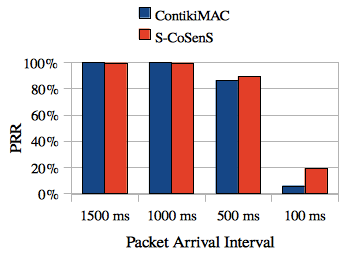
\includegraphics[width=5.25cm]{images/trp-32hz.png}}

{\footnotesize Taux de réception de paquets
                \scriptsize(\nom{TRP}~/ \lang{PRR})}

\end{column}

\begin{column}{5.5cm}

\center{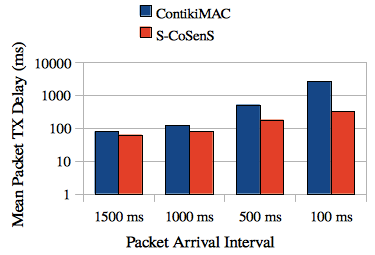
\includegraphics[width=5.25cm]{images/delays-32hz.png}}

{\footnotesize Délais de transmission \lang{end-to-end}}
\end{column}

\end{columns}

\vspace{0.5cm}

\scriptsize{\textbf{Note~:} cycles de 32~Hz~/ 31~ms utilisés pour avoir
 des résultats comparables en termes de TRP entre S-CoSenS et ContikiMAC}

\end{frame}

\begin{frame}[label=comparContikiMAC3]
\frametitle{Comparaison avec ContikiMAC III}
\framesubtitle{Qualité de service (bis)}

\vspace{-0.25cm}

S-CoSenS~/ RIOT largement meilleur que ContikiMAC~/ Contiki~OS en termes
de Qualité de Service (\nom{QdS}) avec des cycles longs~:

\begin{columns}[c]

\begin{column}{5.5cm}

\center{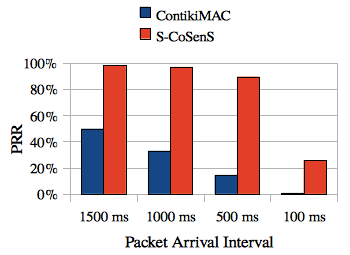
\includegraphics[width=5.25cm]{images/trp-8hz.png}}

{\footnotesize Taux de réception de paquets
                \scriptsize(\nom{TRP}~/ \lang{PRR})}

\end{column}

\begin{column}{5.5cm}

\center{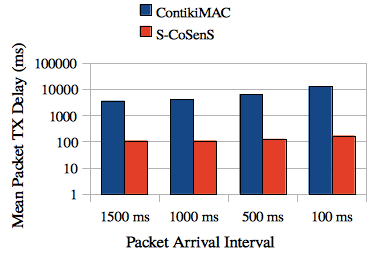
\includegraphics[width=5.25cm]{images/delays-8hz.png}}

{\footnotesize Délais de transmission \lang{end-to-end}}
\end{column}

\end{columns}

\vspace{0.5cm}

\scriptsize{\textbf{Note~:} cycles de 8~Hz~/ 125~ms (durée de cycle
 par défaut pour ContikiMAC)}

\end{frame}

\begin{frame}[label=comparContikiMAC4]
\frametitle{Comparaison avec ContikiMAC IV}
\framesubtitle{Consommation d'énergie (approximation par les
                \lang{duty cycles})}

ContikiMAC~/ Contiki~OS meilleur que S-CoSenS~/ RIOT en termes de
\lang{duty cycles}~:

\vspace{-0.25cm}

\begin{columns}[c]

\begin{column}{5.5cm}

\center{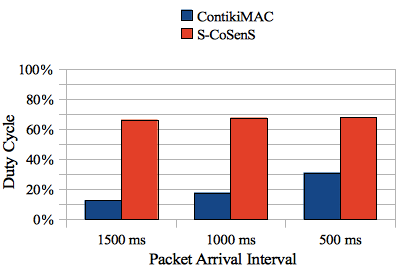
\includegraphics[width=5.5cm]{images/duty-cycles-routeurs.png}}

\footnotesize{\lang{Duty cycles} estimés du n{\oe}ud routeur
               (activité radio totale)}

\end{column}

\begin{column}{5.5cm}

\center{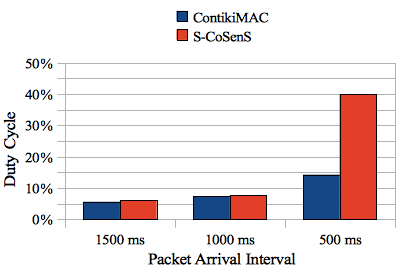
\includegraphics[width=5.5cm]{images/duty-cycles-noeuds-feuilles.png}}

\footnotesize{\lang{Duty cycles} estimés des n{\oe}uds feuilles
               (activité radio totale)}

\end{column}

\end{columns}

\vspace{0.3cm}

\scriptsize{\textbf{Note~:} cycles de 32~Hz~/ 31~ms utilisés pour avoir
 des résultats comparables en termes de TRP entre S-CoSenS et ContikiMAC}

\end{frame}

\begin{frame}[label=comparContikiMAC5]
\frametitle{Comparaison avec ContikiMAC V}
\framesubtitle{Discussion}

\vspace{-0.25cm}

\begin{block}{Constatations issues de ces comparaisons par simulation}
\begin{itemize}
\item S-CoSenS~/ RIOT OS meilleur concernant la Qualité de Service
\item ContikiMAC~/ Contiki OS meilleur concernant les \lang{``duty cycles''}
\item Problèmes de stabilité~: débordements mémoire \\ 
      $\rightarrow$ MPU, ou code de contrôle ajouté au processus
       de compilation
\item Influence de l'implémentation sur les résultats \\
      (cas du pilote de bus SPI sur la transmission des trames)
\item Premières comparaisons avec des tests sur matériel réel \\
      $\rightarrow$ convergence avec nos résultats de simulation~/
       d'émulation
\end{itemize}
\end{block}

\end{frame}


%% 5.4 AMÉLIORATIONS POTENTIELLES DES PROTOCOLES MAC / RDC
\subsection{Améliorations potentielles des protocoles MAC~/ RDC}

\begin{frame}[label=limitesAlgoSCoSenS1]
\frametitle{Limites des algorithmes actuels}
\framesubtitle{Adaptation sub-optimale aux protocoles MAC~/ RDC avancés}

\begin{columns}[c]

\begin{column}{8cm}

\vspace{-0.25cm}
\begin{block}{Cas de S-CoSenS~:}
Trafic estimé par \emph{comptage des paquets transmis}~:\\
\[
\begin{array}{l}
\overline{\mathrm{WP}_n} = \alpha \cdot \overline{\mathrm{WP}_{n - 1}}
                          + (1 - \alpha) \cdot \mathrm{WP}_{n - 1} \\
\mathrm{WP}_n = \mathrm{max}(\mathrm{WP}_{min},
                              \mathrm{min}(\overline{\mathrm{WP}_n},
                                           \mathrm{WP}_{max}))
\end{array}
\]
\begin{itemize}
\item indicateur imparfait (ne voit pas tout le trafic)
\item $\rightarrow$ nécessité d'augmenter $\mathrm{WP}_{min}$
      artificiellement \\
       {\small (cf. \lang{duty cycle} du routeur $\geq 50\%$
                au transparent \pageref{comparContikiMAC4})}
\item $\rightarrow$ idée d'amélioration~: meilleur indicateur...
\end{itemize}
\end{block}

\end{column}

\begin{column}{3.5cm}

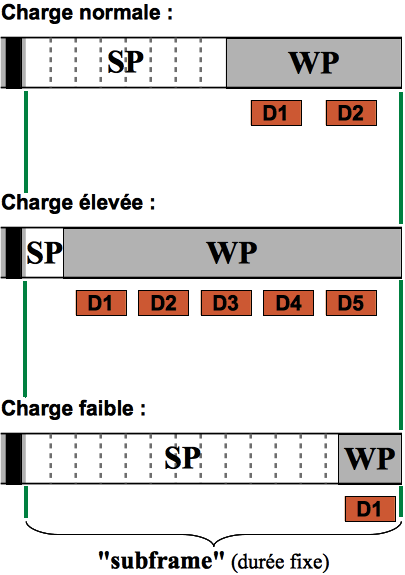
\includegraphics[width=3.5cm]{images/s-cosens-subframe.png}

\end{column}

\end{columns}

\end{frame}

\begin{frame}[label=ameliorAlgo1]
\frametitle{Améliorations algorithmiques des protocoles MAC I}
\framesubtitle{Propositions d'améliorations algorithmiques}

\begin{block}{Proposition d'améliorations algorithmiques des protocoles
               MAC~/ RDC}
\begin{enumerate}
\item \emph{Adaptation du mécanisme de \lang{``phase lock''}} de ContikiMAC
       aux autres protocoles aysnchrones (surtout si cycles de durée fixe)
\item \emph{Comptage des SFD}\footnotemark[1]~--- au lieu des paquets
       retransmis~--- pour mieux \emph{évaluer} le trafic réseau
       (par ex.~: cas de S-CoSenS)
\item \'Etude de \emph{l'influence du rapport signal~/ bruit (SNR)} sur
       les performances des protocoles MAC~/ RDC de tous types
\end{enumerate}
\end{block}

\footnotetext[1]{\scriptsize \nom{SFD~:} \lang{Start-of-Frame Delimiter}
(Signal court suivant le \nom{préambule}, marquant~/ délimitant le début
 d'une trame MAC 802.15.4)}

\end{frame}

\begin{frame}[label=ameliorAlgo2]
\frametitle{Améliorations algorithmiques des protocoles MAC II}
\framesubtitle{Premières évaluations par simulation~/ émulation
                des améliorations proposées}

\vspace{-0.25cm}
\begin{block}{Première évaluation des propositions d'améliorations}

\begin{itemize}
\item \'Evaluations impossibles par simulation~/ émulation
       pour \circleddigit{2} et \circleddigit{3}
\item Première évaluation \emph{exploratoire} via simulation~/
       émulation par Cooja pour \circleddigit{1} avec S-CoSenS
\end{itemize}

\end{block}

{\small
Avec une durée de cycle courte (31~ms), pas d'amélioration significative~:
}

\vspace{-0.25cm}
\center{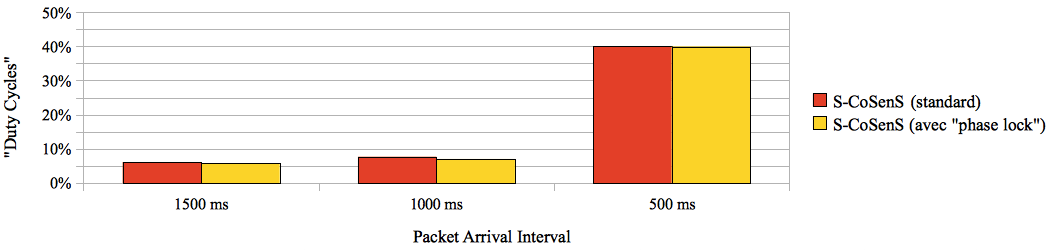
\includegraphics[width=10.75cm]{images/duty-cycles-pl-31ms.png}}

\end{frame}

\begin{frame}[label=ameliorAlgo3]
\frametitle{Améliorations algorithmiques des protocoles MAC III}
\framesubtitle{Résultats des simulations~/ émulations pour l'adaptation
                du \lang{``phase lock''} à S-CoSenS}

\vspace{-0.25cm}
{\small
\begin{itemize}
\item Avec une durée de cycle assez longue (125~ms),
      baisse significative du \lang{duty cycle} de S-CoSenS, mais...
\item ContikiMAC garde toujours un \lang{duty cycle} significativement
      inférieur
\end{itemize}
}

\vspace{-0.5cm}
\center{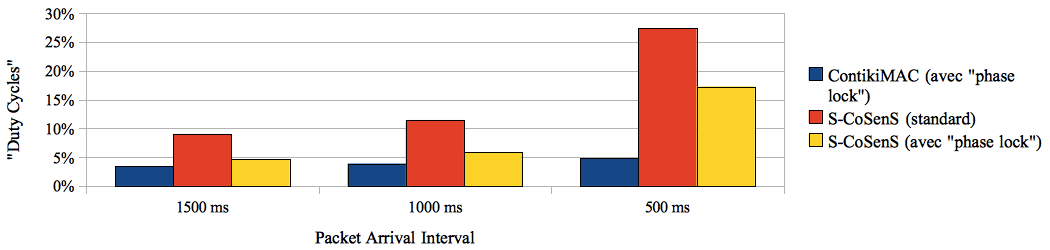
\includegraphics[width=10.75cm]{images/duty-cycles-pl-125ms.png}}

\vspace{-0.25cm}
\begin{exampleblock}{Conclusion}
Mécanisme de \lang{``phase lock''} mieux adapté aux protocoles à durée
de cycle fixe (comme ContikiMAC)
\end{exampleblock}

\end{frame}

%%%%%%%%%%%%%%%%%%%%%%%%%%%%%%%%%%%%%%%%%%%%%%%%%%%%%%%%%%%%%%%%%%%%%%%%%%%%%

%%% SECTION 6 : VALIDATION
\section[Validation sur plates-formes réelles]
        {Validation des expérimentations sur plates-formes réelles}


%% 6.1 MOTIVATION : LIMITATIONS ET INEXACTITUDES DES SIMULATIONS
\subsection{Motivation~: limitations et inexactitudes des simulations}

\begin{frame}[label=Anomalies1]
\frametitle{Anomalies temporelles constatées}
\framesubtitle{Problème au chargement du \lang{buffer} d'envoi de la radio}

Différences constatées entre simulations~/ émulations sous le
\lang{framework} Cooja~/ MSPSim, et tests sur matériel réel~:

\vspace{0.25cm}

\begin{center}
\begin{tabular}{|c|c|r|}
\hline
\textbf{OS} & \textbf{Matériel} & \textbf{Différence moyenne} \\
\hline
\multirow{2}*{Contiki OS}
            & SkyMote~/ TelosB  &   13,0~\% val. exp. \\
            \cline{2-3}
            &    Zolertia Z1    &  110,3~\% val. exp. \\
\hline
\multirow{2}*{RIOT OS}
            & SkyMote~/ TelosB  &   16,3~\% val. exp. \\
            \cline{2-3}
            &    Zolertia Z1    &  183,3~\% val. exp. \\
\hline
\end{tabular}
\end{center}

\vspace{0.25cm}

$\rightarrow$ simulations inadaptées aux évaluations de performances
 (notamment temporelles)

\end{frame}

\begin{frame}[label=Anomalies2]
\frametitle{Conséquences potentielles}

\begin{alertblock}{Conséquences des imprécisions~/ erreurs
                    dans les simulations}
Problèmes de validité des travaux basés sur simulations~/ émulations
pour évaluer les performances~:
\begin{itemize}
\item dans les diverses publications sur le domaine des WSN
\item concernant nos propres travaux de thèse précédents
\end{itemize}

$\rightarrow$ Nécessité de valider sur plates-formes réelles~: matériels
(\lang{``motes''}) suffisamment instrumentés
\end{alertblock}

\begin{exampleblock}{Essais préliminaires sur matériel à base MSP430}
$\rightarrow$ Tendent à valider les conclusions de nos simulations
 précédentes
\end{exampleblock}

\end{frame}


%% 6.2 VALIDATION SUR MATÉRIEL : MOYENS ET OBJECTIFS
\subsection{Validation sur matériel~: moyens et objectifs}

\begin{frame}[label=Validation1]
\frametitle{Projets de tests de validation I}

\begin{block}{Premier but~: valider nos expériences précédentes}
\begin{itemize}
\item Validation de notre implémentation de S-CoSenS
\item \'Evaluation de ses performances via comparaison avec ContikiMAC
\end{itemize}
\end{block}

\end{frame}

\begin{frame}[label=Validation2]
\frametitle{Projets de tests de validation II}

\vspace{-0.25cm}

\begin{block}{Second but~: tester la montée en charge~:}
$\rightarrow$ Réseau étendu, comportant 4 PAN et 5 routeurs
\end{block}

\vspace{-0.25cm}
\center{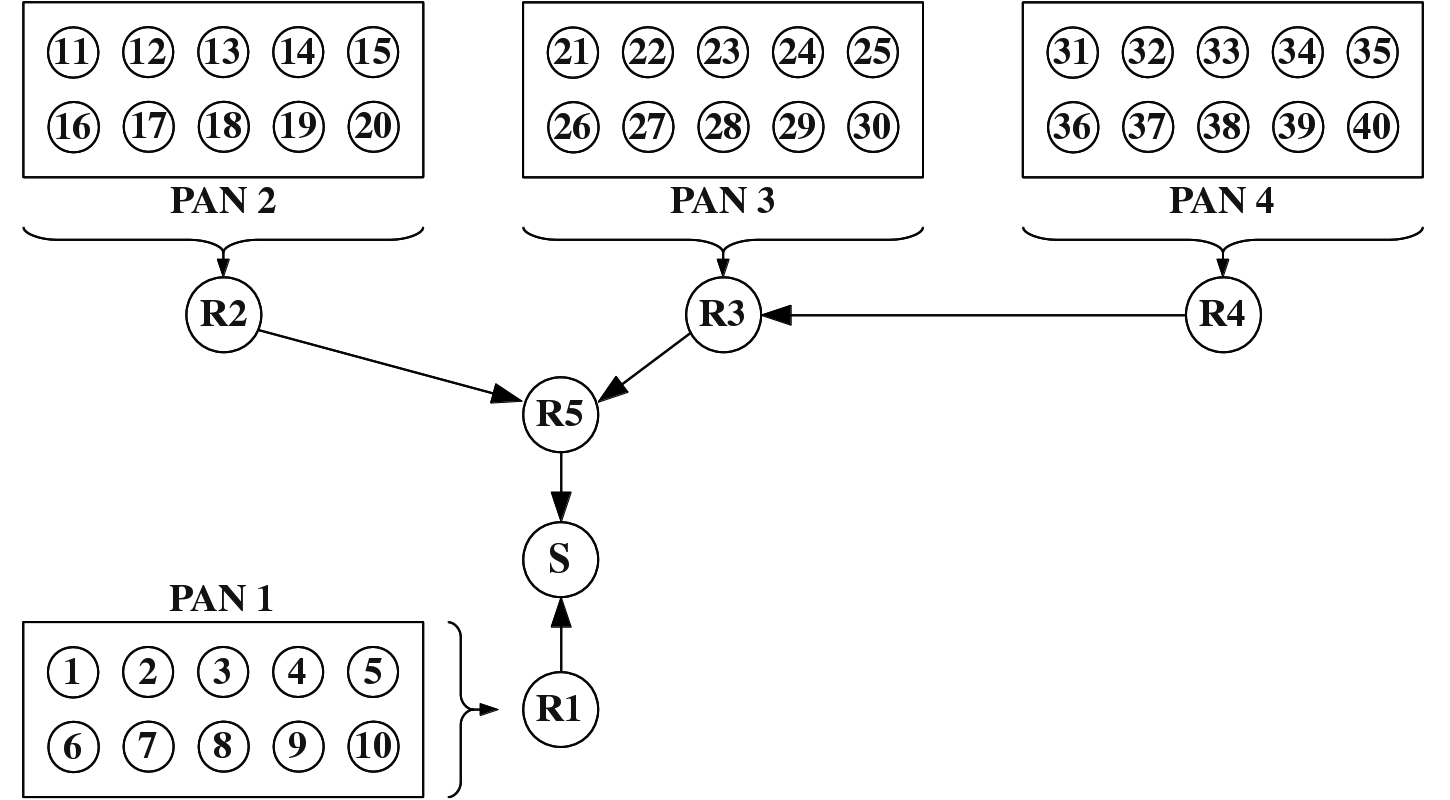
\includegraphics[width=8.5cm]{images/config-test-2.png}}

\end{frame}

\begin{frame}[label=Validation3]
\frametitle{Plate-forme de tests}

\vspace{-0.25cm}
\begin{block}{Choix de la plate-forme matérielle d'expérimentation}
\begin{itemize}
\item Besoin d'un \lang{testbed} offrant suffisamment de n{\oe}uds
       disponibles, \emph{avec possibilités d'instrumentation} adaptées
\item Choix retenu~= plate-forme \nom{IoT-LAB}, n{\oe}uds de type M3, car~:
  \begin{itemize}
  \item performants (MCU ARM Cortex-M3 $\rightarrow$ puissance de calcul
         et espace~mémoire supérieurs)
  \item assez instrumentés (\lang{sniffer} de paquets avec horodatage,
         consommation énergétique, sortie console...)
  \end{itemize}
\end{itemize}
\end{block}

\begin{alertblock}{Problème constaté sur IoT-LAB~:}
\lang{Sniffer} de paquets pas assez précis pour toujours détecter
les trames d'acquittement (\nom{ACK})~!
\end{alertblock}

\end{frame}


%% 6.3 TRAVAUX ET MISE EN OEUVRE
\subsection{Travaux et mise en {\oe}uvre}

\begin{frame}[label=Problemes1]
\frametitle{Problèmes techniques rencontrés}

\begin{block}{Fin des travaux de validation dans le cadre de la thèse}
\begin{itemize}
\item Multiples problèmes techniques \\
      $\rightarrow$ principalement <<~surdité~>> récurrente des n{\oe}uds
\item Pas d'explication satisfaisante
  \begin{itemize}
  \item bogue logiciel~?
  \item problème matériel (\lang{``brownout''})~?
  \end{itemize}
 malgré plusieurs mois d'essais et de déboguage infructueux
\item Tests de validation impossibles à mener à terme
\item Notre réaction et contribution~: \emph{description technique aussi
détaillée que possible des problèmes rencontrés, afin de faciliter
la résolution de ces problèmes dans des travaux ultérieurs.}
\end{itemize}

\end{block}

\end{frame}

%%%%%%%%%%%%%%%%%%%%%%%%%%%%%%%%%%%%%%%%%%%%%%%%%%%%%%%%%%%%%%%%%%%%%%%%%%%%%

%%% SECTION 7 : CONCLUSION ET PERSPECTIVES
\section{Conclusions et perspectives}


%% 7.1 CONCLUSIONS GÉNÉRALES :  RÉSUMÉ DES CONTRIBUTIONS DE LA THÈSE
\subsection{Conclusions générales}

\begin{frame}[label=ConclusionsContribs1]
\frametitle{Contributions I}
\framesubtitle{Résumé des contributions de la thèse...}

\begin{exampleblock}{Multiples contributions sur plusieurs domaines~:}
\begin{itemize}
\item OS spécialisés dans les WSN~/ couches basses de leurs piles
       protocolaires réseau~:
  \begin{itemize}
  \item évaluation des principales plates-formes logicielles disponibles
  \item contributions techniques~: travail sur une plate-forme logicielle
        pour implanter fonctionnalités et robustesse requises
  \item démonstration de la nécessité de fonctionnalités temps-réel
  \end{itemize}
\item Idées d'améliorations algorithmiques des protocoles MAC~/ RDC
\item Démonstration~: tout exécutable ELF (dont RIOT OS) peut fonctionner
       sous Cooja 
\end{itemize}
\end{exampleblock}

\end{frame}

\begin{frame}[label=ConclusionsContribs2]
\frametitle{Contributions II}
\framesubtitle{Résumé des contributions de la thèse (suite et fin)}

\begin{exampleblock}{Multiples contributions sur plusieurs domaines
                     (suite et fin)}
\begin{itemize}
\item Découverte et description d'un bogue de \lang{timing} dans MSPSim \\
      $\rightarrow$ code de test publié sur Github
\item Limites des simulations~/ émulations \\ 
      $\rightarrow$ nécessité de valider les évaluations sur matériel réel
\item Description aussi détaillée que possible des problèmes techniques
      rencontrés et non résolus dans le manuscrit \\
      $\rightarrow$ But~: permettre la résolution des difficultés et la
       réussite des expériences prévues dans des travaux ultérieurs
\end{itemize}
\end{exampleblock}

\end{frame}

\begin{frame}[label=ConclusionsContribs3]
\frametitle{Conclusion générale}

\vspace{-0.25cm}
\begin{alertblock}{Conclusions de notre Thèse~:}
\emph{Nous avons démontré~:}
\begin{itemize}
\item \emph{la possibilité d'implémenter des protocoles MAC~/ RDC~:}
  \begin{itemize}
  \item \emph{s'adaptant dynamiquement aux trafics réseau,}
  \item \emph{offrant les meilleurs compromis QdS~/ consommation d'énergie,}
  \item \emph{privilégiant une QdS optimale~;}
  \end{itemize}
  \emph{$\rightarrow$ de façon à la fois efficace, portable
        et standardisée}
\item \emph{la nécessité d'un OS dédié WSN~:}
  \begin{itemize}
  \item \emph{pour portabilité, facilité de développement et standardisation,}
  \item \emph{offrant les fonctionnalités requises (temps-réel).}
  \end{itemize}
\end{itemize}
\emph{Indispensable pour traiter des données sensibles et prioritaires~: \\
cas de l'e-santé (projet LAR, détection d'urgences...)~!}
\end{alertblock}

\end{frame}


%% 7.2 PERSPECTIVES
\subsection{Perspectives}

\begin{frame}[label=Perspectives1]
\frametitle{Perspectives I}

\begin{block}{Terminer les travaux prévus sur matériel}
\begin{itemize}
\item Résolution des problèmes (autre plate-forme matérielle de test)
\item Adaptation de nos protocoles MAC~/ RDC avancés (S-CoSenS, iQueueMAC)
       à la pile \texttt{gnrc} de RIOT OS
\item Tests sur matériel~:
  \begin{itemize}
  \item validation des travaux de la thèse faits par simulation~/
         émulation
  \item évaluation des améliorations algorithmiques proposées
         (SFD, SNR) sur la couche MAC
  \item tests de montée en charge (réseaux complexes~: multi-PAN...)
  \end{itemize}
\end{itemize}

\end{block}

\end{frame}

\begin{frame}[label=Perspectives2]
\frametitle{Perspectives II}

\begin{exampleblock}{Influence de la PF logicielle sur la couche MAC}
Influence de RIOT OS sur les performances de protocoles MAC~/ RDC avancés~?

\medskip

$\rightarrow$ Collaboration en cours avec S.~Zhuo, pour intégrer
nos travaux dans la pile \texttt{gnrc} de RIOT OS~:
\begin{itemize}
\item modules CSMA~/ CA et MAC IEEE 802.15.4 en cours de
tests sur une autre PF matérielle (cartes SAMR21 Xplained Pro) \\
$\rightarrow$ bientôt intégrés dans RIOT~?...
\item protocoles MAC~/ RDC avancés~: développement en cours...
\end{itemize}
\end{exampleblock}

\end{frame}

\begin{frame}[label=Idees1]
\frametitle{Constats et idées d'amélioration}

\vspace{-0.25cm}

\begin{block}{Influence de la conception des composants
              sur les capteurs sans-fil~:}
\begin{itemize}
\item Limitations gênantes, pour les WSN, des MCU courants \\ 
      $\rightarrow$ la première~: manque de RAM
\item Intégration de l'émetteur~/ récepteur radio
  \begin{itemize}
  \item Avantage~: facilite programmation et déboguage
  \item Inconvénient~: pas de choix pour l'émetteur~/ récepteur radio
  \end{itemize}
\end{itemize}
\end{block}

\begin{block}{}
\begin{itemize}
\item Encore peu de composants \emph{spécifiques} dédiés aux capteurs
sans-fil...
\item ... Mais les industriels y viennent
{\small(ex.~: Atmel~AVR ATmegaRFR2, TI~ChipCon SensorTags...)}
\item Utilisation de FPGA pour développer des SoC dédiés aux WSN~?
(exemple du projet NetFPGA, lancé depuis déjà 2007)
\end{itemize}
\end{block}

\end{frame}

%%%%%%%%%%%%%%%%%%%%%%%%%%%%%%%%%%%%%%%%%%%%%%%%%%%%%%%%%%%%%%%%%%%%%%%%%%%%%

%% DIAPO. FINALE

\section*{}

\begin{frame}[label=Finale]
\frametitle{Merci de votre attention}

% Faire un point d'interrogation "stylé" !
\pgfdeclareradialshading{goldball}{\pgfpoint{0.5mm}{0.5mm}}{
  rgb(0mm)=(0.9,0.8,0);
  rgb(0.7mm)=(0.7,0.6,0);
  rgb(1mm)=(0.5,0.4,0);
  rgb(1.05mm)=(1,1,1)
}
\newcommand{\goldchar}{%
  \begin{pgfpicture}{-1ex}{-0.65ex}{1.5ex}{1.5ex}%
  {\pgftransformscale{5}\pgftext{\normalsize\pgfuseshading{goldball}}}%
  {\pgfsetfillcolor{darkgray!75!gray}\Huge\bfseries%
   \pgftext{\foreignlanguage{english}{?}}}%
  \end{pgfpicture}%
}
\center{\Large \textbf{Questions}\hspace{5mm}\goldchar}

\end{frame}

%%%%%%%%%%%%%%%%%%%%%%%%%%%%%%%%%%%%%%%%%%%%%%%%%%%%%%%%%%%%%%%%%%%%%%%%%%%%%

\setbeamertemplate{navigation symbols}{}
\appendix

%%% ANNEXE : PUBLICATIONS

\section{Annexe~: Publications et réalisations}


\subsection{Publications scientifiques}

\begin{frame}[label=publis]
\frametitle{Publications scientifiques}

\tiny

\textbf{Conférences~/ \lang{``workshops''}}
\begin{itemize}
\item Moutie Chehaider, Kévin Roussel, Ye-Qiong Song.
<<~Interopérabilité des réseaux de capteurs hétérogènes dans
un appartement intelligent~>>
\textit{9èmes journées francophones Mobilité et Ubiquité}, UbiMob 2013.
Nancy, France. Juin 2013.
\item Kévin Roussel.
<<~Implementing a real-time MAC protocol under RIOT OS : running on
Zolertia Z1 motes~>>
In \textit{Workshop Internet of Things / Equipex FIT IoT-LAB},
INRIA Grenoble Rhone-Alpes, Montbonnot, France. Novembre 2014.
(présentation sans actes.)
\item Kévin Roussel, Ye-Qiong Song, Olivier Zendra.
<<~RIOT OS Paves the Way for Implementation of High-performance
MAC Protocols~>>
In \textit{Proceedings of the 4th International Conference
on Sensor Networks}, SensorNets 2015, pages 5--14.
ESEO, Angers, France. Février 2015.
\item Kévin Roussel, Ye-Qiong Song, Olivier Zendra.
<<~ Using Cooja for WSN Simulations: Some New Uses and Limits ~>>.
In \textit{Proceedings of the 2016 International Conference on Embedded
Wireless Systems and Networks}~--- EWSN~'16~; \lang{workshop NextMote},
pages 319--324.
\lang{Technische Universit\"at}, Graz, Autriche. Février 2016.
\end{itemize}

\textbf{Rapports de recherche INRIA (HAL)}
\begin{itemize}
\item Kévin Roussel, Ye-Qiong Song.
<<~A critical analysis of Contiki's network stack for integrating
new MAC protocols~>>. 13 pages. Décembre 2013.\\
Rapport de recherche INRIA \no~8776 \textit{(CRI-Nancy Grand Est)}.\\
ID hal-01202542.
\item Kévin Roussel, Ye-Qiong Song, Olivier Zendra.
<<~Practical Lessons Learned through Implementation and Performance
Evaluation of Two MAC/RDC Protocols on WSN OS~>> 25 pages. Mars 2015.\\
Rapport de recherche INRIA \no~8777 \textit{(CRI-Nancy Grand Est)}.\\
ID hal-01202664.
\end{itemize}

\end{frame}


\subsection{Réalisations techniques}

\begin{frame}[allowframebreaks]  %% nombreuses références :) ...
\frametitle{Réalisations techniques}
\framesubtitle{``Pull Requests'' sur GitHub}

\tiny

\textbf{Pour Contiki OS}
Ces deux contributions ont été refusées (mais réutilisées en partie et
indirectement pour une amélioration ultérieure de l'API radio de Contiki~:
PR \#617 de Niklas Finne et~al, intégrée au code de Contiki OS en juin 2014).

\begin{itemize}
\item Kévin Roussel, George Oikonomou, Mariano Alvira, David Kopf,
      Valentin Sawadski, Joakim Eriksson, Peter A. Bigot, Adam Dunkels.
PR \#192~: <<~Extended radio drivers API~>>.
(2013--2014).
\item Kévin Roussel, Mariano Alvira, Joakim Eriksson, George Oikonomou,
      Oliver Schmidt, Adam Dunkels, Nicolas Tsiftes.
PR \#519~: <<~Radio api extension~>>.
(2014).
\end{itemize}

\textbf{Pour RIOT OS}
Toutes les contributions citées ci-dessous dans la présente section
ont été acceptées et ont été intégrées (\lang{``merged PRs''})
à la branche principale du code de RIOT OS.

\begin{itemize}
\item Kévin Roussel, Ludwig Knüpfer, Oliver Hahm, Thomas Eichinger.
PR \#408~: <<~Simplify msp430 headers~>>
(2013).
\item Kévin Roussel, Oliver Hahm, Ludwig Knüpfer.
PR \#459~: <<~Msp430 lpm freq~>>
(2013--2014).
\item Kévin Roussel, Oliver Hahm, Kaspar Schleiser, Ludwig Knüpfer,
      Christian Mehlis, René Kijewski.
PR \#685~: <<~Panic~>>
(2014).\\
\emph{Best PR award of the month (Février 2014).}

\item Kévin Roussel, René Kijewski, Oliver Hahm, Ludwig Knüpfer,
      Christian Mehlis.
PR \#687~: <<~Add a \texttt{reboot()} function to \texttt{kernel.h}
              definitions~>>
(2014).
\item Kévin Roussel, René Kijewski, Kaspar Schleiser.
PR \#689~: <<~Portable definition of function attributes~>>
(2014).
\item Kévin Roussel, René Kijewski, Oliver Hahm, Ludwig Knüpfer.
PR \#724~: <<~Reboot~>>
(2014).
\item Kévin Roussel, René Kijewski, Oliver Hahm.
PR \#881~: <<~Ensure that stack pointer is correcty aligned during
              thread creation on MSP430~>>
(2014).
\item Kévin Roussel, Oliver Hahm, Thomas Eichinger.
PR \#882~: <<~CC2420 radio tranceiver's driver fixes~>>
(2014).
\item Kévin Roussel, Oliver Hahm, Ludwig Knüpfer, Christian Mehlis,
      Thomas Eichinger, Hauke Petersen.
PR \#893~: <<~Zolertia Z1 port for RIOT OS~>>
(2014).
\item Kévin Roussel, Ludwig Knüpfer, Thomas Eichinger, Oliver Hahm,
      René Kijewski.
PR \#915~: <<~Add a standard way to query CCA status on CC2420 transceiver~>>
(2014).
\item Kévin Roussel, Oliver Hahm, Ludwig Knüpfer, Thomas Eichinger,
      Martine Lenders, Hauke Petersen.
PR \#925~: <<~Proposal for common 802.15.4 radio driver API definition~>>
(2014).
\item Kévin Roussel, Oliver Hahm.
PR \#954~: <<~Fix for CC2420 radio driver for TelosB~>>
(2014).
\item Kévin Roussel, Oliver Hahm, Ludwig Knüpfer.
PR \#957~: <<~Handle race conditions preventing MSP430 timers to be set
              correctly~>>
(2014).
\item Kévin Roussel, René Kijewski, Kaspar Schleiser, Ludwig Knüpfer,
      Oliver Hahm, Christian Mehlis.
PR \#970~: <<~core: Add the ability to send a message to the current
              thread's message queue~>>
(2014).
\item Kévin Roussel, Ludwig Knüpfer, René Kijewski, Oliver Hahm,
      Christian Mehlis, Kaspar Schleiser.
PR \#1002~: <<~Enhance implementation of \texttt{hwtimer\_ spin()}~>>
(2014).
\item Kévin Roussel, Oliver Hahm, Ludwig Knüpfer.
PR \#1113~: <<~Use Timer B on MSP430 architecture~>>
(2014).
\item Kévin Roussel, Oliver Hahm.
PR \#1211~: <<~Completing low-level radio driver definition~>>
(2014).
\item Kévin Roussel, Oliver Hahm, Thomas Eichinger, Christian Mehlis.
PR \#1223~: <<~Modify \& extend CC2420 driver to comply with API described
               in \texttt{radio\_ driver.h}~>>
(2014).
\item Kévin Roussel, Oliver Hahm.
PR \#1239~: <<~Add a missing constant in \texttt{'radio\_ tx\_status\_t'}
               enum~>>
(2014).
\item Kévin Roussel, René Kijewski, Hauke Petersen, Ludwig Knüpfer,
      Christian Mehlis, Oliver Hahm.
PR \#1380~: <<~Reset ARM Cortex-M3 MCUs before flashing~>>
(2014).
\item Kévin Roussel, Ludwig Knüpfer, Oliver Hahm.
PR \#1383~: <<~Fix a design error in \texttt{cc2420\_do\_send()} function~>>
(2014).
\item Kévin Roussel, Ludwig Knüpfer, Oliver Hahm.
PR \#1385~: <<~Fix a nasty race condition in CCA determination on CC2420~>>
(2014).
\item Kévin Roussel, Oliver Hahm.
PR \#1388~: <<~boards/z1: fix \texttt{cc2420\_txrx} function in CC2420
               driver HAL~>>
(2014).
\item Kévin Roussel, Ludwig Knüpfer, Hauke Petersen, Kaspar Schleiser.
PR \#1617~: <<~Ensure \texttt{hwtimer\_spin()} won't wait for
               an unreachable stop counter value~>>
(2014).
\item Kévin Roussel, Ludwig Knüpfer, Oliver Hahm, Hinnerk van Bruinehsen.
PR \#1618~: <<~Fix \texttt{thread\_yield()} on MSP430 platforms~>>
(2014).
\item Kévin Roussel, Ludwig Knüpfer, Oliver Hahm, Hinnerk van Bruinehsen,
      Martine Lenders.
PR \#1619~: <<~Only use 16 significative bits for MSP430 \texttt{hwtimer}s~>>
(2014).
\item Kévin Roussel, Oliver Hahm, Ludwig Knüpfer.
PR \#2214~: <<~Msp430 misc interrupt-related fixes~>>
(2014).
\item Kévin Roussel, Jonas Remmert, Oliver Hahm
PR \#4138~: <<~Add a \texttt{netopt} for getting and setting CCA threshold~>>
(2015).

\end{itemize}
\end{frame}


%%%%%%%%%%%%%%%%%%%%%%%%%%%%%%%%%%%%%%%%%%%%%%%%%%%%%%%%%%%%%%%%%%%%%%%%%%%%%

%%% FIN DE LA PRÉSENTATION

\section*{}

\begin{frame}

\centering{\LARGE\itshape
           \foreignlanguage{english}{``That's all Folks!''}}

\end{frame}


%%%%%%%%%%%%%%%%%%%%%%%%%%%%%%%%%%%%%%%%%%%%%%%%%%%%%%%%%%%%%%%%%%%%%%%%%%%%%%%%
%%%                               80 COLONNES                                %%%
%%%%%%%%%%%%%%%%%%%%%%%%%%%%%%%%%%%%%%%%%%%%%%%%%%%%%%%%%%%%%%%%%%%%%%%%%%%%%%%%

\end{document}

